\documentclass{article}

\usepackage{graphicx}			% Provides graphics utilities
\graphicspath{ {figures/} }		% Sets graphics path
\usepackage{pdfpages}   		% Allows pdfs to be inserte into this document
\usepackage[hyphens]{url}		% Breaks long URLs across lines

% Load last
\usepackage{hyperref}			% Makes hyperlinks in .pdf output


\bibliographystyle{abbrv}

\begin{document}

%%%%%%%%%%%%%%%%%%%%%%%%%%%%%%%%%%%%%%%%%%%%%%%%%%%%%%%%%%%%%%
\title{Git Branching Strategy}
\author{Matthew Kuperus Heun}
%%%%%%%%%%%%%%%%%%%%%%%%%%%%%%%%%%%%%%%%%%%%%%%%%%%%%%%%%%%%%%

\maketitle


%%%%%%%%%%%%%%%%%%%%%%%%%%%%%%%%%%%%%%%%%%%%%%%%%%%%%%%%%%%%%%
\begin{abstract}
%%%%%%%%%%%%%%%%%%%%%%%%%%%%%%%%%%%%%%%%%%%%%%%%%%%%%%%%%%%%%%

This document gives my strategy for branching in a git repository. 
The strategy is based on the fine blog post by Vincent Driessen
and other resources.
Adherence to this strategy will enable better development processes.
\end{abstract}


%%%%%%%%%%%%%%%%%%%%%%%%%%%%%%%%%%%%%%%%%%%%%%%%%%%%%%%%%%%%%%
\section{Introduction} 
\label{sec:introduction}
%%%%%%%%%%%%%%%%%%%%%%%%%%%%%%%%%%%%%%%%%%%%%%%%%%%%%%%%%%%%%%

The use of branches can greatly assist software development projects, 
particularly when developers need to both 
work on new features and maintain released code.

This document gives my model for branching in a git repository. 
The strategy is based on the fine blog post by Vincent Driessen~\cite{Driessen:2010}
and other resources~\cite{Onkelinx:2017, Rankin:2010}.
The model assumes the existence of \texttt{github} or a similar remote repository
and use of the RStudio IDE, 
although the model (if not the details) 
will apply to other IDEs that support branching. 

In addition, it can be difficult to remember 
all of the \texttt{git} commands for branching and merging.
This document gathers all commands in a single place
and discusses the commands in the context of the overall workflow.
 
Adherence to this strategy and use of these commands 
will improve my software development processes.


%%%%%%%%%%%%%%%%%%%%%%%%%%%%%%%%%%%%%%%%%%%%%%%%%%%%%%%%%%%%%%
\section{Rules} 
\label{sec:rules}
%%%%%%%%%%%%%%%%%%%%%%%%%%%%%%%%%%%%%%%%%%%%%%%%%%%%%%%%%%%%%%

\begin{enumerate}

  \item The \texttt{master} and \texttt{develop} branches are persistant
  
  \item Only one (1) \texttt{release-x.x.x} branch can exist at any given time

  \item Only one (1) \texttt{hotfix-x.x.x} branch can exist at any given time
  
  \item Any number of feature branches can co-exist
  
  \item Releases are retrieved by reverting to tags

\end{enumerate}


%%%%%%%%%%%%%%%%%%%%%%%%%%%%%%%%%%%%%%%%%%%%%%%%%%%%%%%%%%%%%%
\section{Workflows} 
\label{sec:workflows}
%%%%%%%%%%%%%%%%%%%%%%%%%%%%%%%%%%%%%%%%%%%%%%%%%%%%%%%%%%%%%%

The workflows presented here assume familiarity 
with the Driessen branching model~\cite{Driessen:2010}. 
(See attached figure.)
All \texttt{git} commands must be entered 
at the command line of the developer's local computer
in the root directory of the repository.
Both Terminal.app (MacOS) and the Terminal window of RStudio
can be used for this purpose.


%++++++++++++++++++++++++++++++
\subsection{Setup} 
\label{sec:setup}
%++++++++++++++++++++++++++++++

Use the following workflow to establish a repository and 
create the \texttt{master} (release) and \texttt{develop} branches.
%
\begin{enumerate}

  \item Create a git repository

  \item Clone the repository, duplicating the \texttt{master} branch on the local computer:
  		\texttt{git clone git@github.com:MatthewHeun/<<RepositoryName>>.git}
  
  \item Create the \texttt{develop} branch: 
  		\texttt{git checkout -b develop master}
		
  \item Make an initial push of the \texttt{develop} branch to origin (github):
        \texttt{git push -u origin develop}
		
  \item Future pushes to github from the \texttt{develop} branch 
  		can be made from RStudio's \texttt{git interface}.

  \item If needed, click the refresh icon 
  		(\raisebox{-0.3\height}{
\includegraphics[scale=0.5]{refresh}}) in the Git pane of RStudio to 
  		show that the project is now on the \texttt{develop} branch.
  
\end{enumerate}


%++++++++++++++++++++++++++++++
\subsection{Develop a feature (\texttt{newfeature})} 
\label{sec:feature}
%++++++++++++++++++++++++++++++

Use the following steps to develop a feature.

\begin{enumerate}

  \item Switch to develop branch: \texttt{git checkout develop}

  \item Create a feature branch: \texttt{git checkout -b newfeature develop} 
  
  \item Work on the feature
  
  \item Add new features to \texttt{NEWS.md} file as they are developed, but
        don't add a version number or date yet.

  \item Commit changes locally

  \item If \texttt{newfeature} is to be pushed to github, RStudio won't be able to do so until you
  %
  \begin{enumerate}

    \item Make an initial push of the \texttt{newfeature} branch
	      to the origin (github):
		  \texttt{git push -u origin newfeature} 
	
	\item Future pushes to github can be made using the RStudio interface.

  \end{enumerate}
  %
  \item When complete, merge \texttt{newfeature} with the \texttt{develop} branch:
  %
  \begin{enumerate}

    \item Switch to develop branch: \texttt{git checkout develop}

    \item Merge \texttt{newfeature} into develop: \texttt{git merge --no-ff newfeature}
	
	\item Add a commit comment (or accept the default) using \texttt{vi} 
	
	\item Save the comment using \texttt{ZZ} (``save'' in \texttt{vi})

  \end{enumerate}
  %
  \item If needed, click the refresh icon 
		(\raisebox{-0.3\height}{
\includegraphics[scale=0.5]{refresh}}) to show that the 
		changes have been merged properly.
  
  \item Push changes on \texttt{develop} branch to github
  %
  \item When satisfied, delete \texttt{newfeature} branch
  %
  \begin{enumerate}

    \item Switch to develop branch: \texttt{git checkout develop}

    \item Delete locally: \texttt{git branch -d newfeature}

    \item Delete remote (if necessary): \texttt{git push -d origin newfeature} 
	
	\item Prune from other machines (if necessary): \texttt{git remote prune origin} 

  \end{enumerate}
  
  \item If intending to submit to CRAN, 
        run the following steps.
  
  \begin{enumerate}
	  
    \item \verb+devtools::spell_check()+

	\item \verb+devtools::check_win_release()+

    \item \verb+devtools::check_win_devel()+

    \item \verb+devtools::check_rhub(interactive = FALSE)+
	
    \item \verb+revdepcheck::revdep_check(num_workers = 4)+
    %
    \begin{enumerate}

      \item Note that \texttt{revdepcheck} must be installed from github. 
            See \url{https://github.com/r-lib/revdepcheck}.

      \item \texttt{source("https://install-github.me/r-lib/revdepcheck")}

    \end{enumerate}
    %

    \item \verb+devtools::release()+ \\
          But don't actually release to CRAN!
            
  \end{enumerate}
  %
\end{enumerate}


%++++++++++++++++++++++++++++++
\subsection{Prepare for release} 
\label{sec:prep-for-release}
%++++++++++++++++++++++++++++++

Use the following steps to prepare for a release.

\begin{enumerate}

  \item Switch to develop branch: \texttt{git checkout develop}

  \item Create a release branch: \texttt{git checkout -b release-x.x.x develop} 

  \item If the \texttt{release-x.x.x} branch is to be pushed to github
        (necessary if you want to submit to CRAN), 
        RStudio won't be able to do so until you
  %
  \begin{enumerate}

    \item Commit locally

    \item Make an initial push of the \texttt{release-x.x.x} branch
	      to the origin (github): 
		  \texttt{git push -u origin release-x.x.x} 
	
	\item Future pushes to github can be made using the RStudio interface.

  \end{enumerate}
  %
  \item Update documentation to reflect new version (\texttt{x.x.x}) and date.
        At a minimum:
  %
  \begin{enumerate}

    \item Update \texttt{DESCRIPTION}, including \texttt{Version:} and \texttt{Date:} fields 
	
    \item Update \texttt{NEWS.md} with version number, date, and release notes
    
	\item Update \texttt{inst/CITATION} version number 
	      in \texttt{note} and \texttt{textVersion} fields.
		  
    \item Update \texttt{cran-comments.md} if submitting to CRAN.

    \item \texttt{cmd-shift-B} to build the package
	
    \item \texttt{cmd-shift-T} to test the package
	
    \item \verb!devtools::test_coverage()! to compute test coverage

	\item \texttt{cmd-shift-E} to check the package
	
	\item \texttt{cmd-shift-W} to update the GitHub pages website 
	      with new version number and documentation.
		  
  \end{enumerate}
  %
  \item Commit locally
  
  \item Optionally, push to GitHub

\end{enumerate}


%++++++++++++++++++++++++++++++
\subsection{Release} 
\label{sec:release}
%++++++++++++++++++++++++++++++

Use the following steps to release a new version (\texttt{x.x.x}).

\begin{enumerate}

  \item If submitting to CRAN:
  
	\begin{enumerate}
	  
	  \item \verb+devtools::spell_check()+

	  \item \verb+devtools::check_win_release()+
	  
	  \item \verb+devtools::check_win_devel()+

	  \item \verb+devtools::check_rhub(interactive = FALSE)+

	  \item \verb+revdepcheck::revdep_check(num_workers = 4)+

	  \item \verb+devtools::release()+ \\
            If \texttt{ERROR: No upstream branch} occurs, 
            push the \texttt{release-x.x.x} branch to GitHub using
            \texttt{git push -u origin release-x.x.x}
        
      \item Answer all questions
      
      \item Verify submission to CRAN (via email)
	  
	  \item Wait for email acknowledging package is on its way to CRAN
            
	\end{enumerate}
  %
  \item Merge \texttt{release-x.x.x} into \texttt{master}
  %
  \begin{enumerate}

    \item Switch to master branch: \texttt{git checkout master} 

    \item Perform merge: \texttt{git merge --no-ff release-x.x.x}
	
	\item Add a commit comment (or accept the default) using \texttt{vi} 
	
	\item Save the comment using \texttt{ZZ} (``save'' in \texttt{vi})
	
  \end{enumerate}
  %
  \item Push \texttt{master} to github
  
  \item Tag the release
  %
  \begin{enumerate}

    \item Tag local: \texttt{git tag -a vx.x.x}

    \item Tag remote (github)
	%
	\begin{enumerate}

	  \item Navigate to github page for the repository\\
	  		(\texttt{http://github.com/MatthewHeun/<<RepositoryName>>})

	  \item Click the releases button (\raisebox{-0.3\height}{
\includegraphics[scale=0.5]{releases_button}})
	  
	  \item Create a new release

	\end{enumerate}
	%
	\item Tag admin
	%
	\begin{enumerate}

	  \item List local tags: \texttt{git tag -l}.
	
	  \item List remote tags: \texttt{git ls-remote --tags origin}.

	  \item Pull remote tags to local repo: \texttt{git fetch --tags}.
	
	  \item Check out at a tag: \texttt{git checkout tags/vx.x.x}.

	\end{enumerate}
	%
  \end{enumerate}
  %
  \item Merge \texttt{release-x.x.x} into \texttt{develop} branch
  %
  \begin{enumerate}

	\item Switch to develop branch: \texttt{git checkout develop}

    \item Perform merge: \texttt{git merge --no-ff release-x.x.x}
	
	\item Add a commit comment (or accept the default) using \texttt{vi} 
	
	\item Save the comment using \texttt{ZZ} (``save'' in \texttt{vi})

  \end{enumerate}
  %
  \item Fix any conflicts that arise in the \texttt{develop} branch
  
  \item Push \texttt{develop} branch to github
  
  \item When satisfied, delete \texttt{release-x.x.x} branch
  %
  \begin{enumerate}

    \item Switch to develop branch: \texttt{git checkout develop}

    \item Delete locally: \texttt{git branch -d release-x.x.x}

    \item Delete remote (if necessary): \texttt{git push -d origin release-x.x.x} 
	
	\item Prune from other machines (if necessary): \texttt{git remote prune origin} 

  \end{enumerate}
  
\end{enumerate}


%++++++++++++++++++++++++++++++
\subsection{Perform a hotfix} 
\label{sec:hotfix}
%++++++++++++++++++++++++++++++

Execute the following steps to perform a hotfix to the current release.

\begin{enumerate}

  \item Switch to master branch: \texttt{git checkout -b master} 

  \item Create hotfix branch: \texttt{git checkout -b hotfix-x.x.x master} 
	
  \item Develop the fix
	
  \item Update documentation to reflect new version (\texttt{x.x.x}) and date.
        At a minimum:
  %
  \begin{enumerate}

    \item Update \texttt{DESCRIPTION}, including \texttt{Version:} and \texttt{Date:} fields 

    \item Update \texttt{NEWS.md} with release notes
	
	\item Re-run \texttt{cmd-shift-W} or \texttt{Build pkgdown} from Addins menu or \\
		  \verb#pkgdown:::build_site_external()# at the command line.
		  This step updates the version number on \texttt{pkgdown} website documentation. 

  \end{enumerate}
  %  
  \item Prepare release notes
  
  \item Commit locally
	
  \item If \texttt{hotfix-x.x.x} is to be pushed to github, RStudio won't be able to do so until you
  %
  \begin{enumerate}

    \item Make an initial push of the \texttt{hotfix-x.x.x} branch
  	      to the origin (github):
  		  \texttt{git push -u origin hotfix-x.x.x} 
		  
	\item If needed, click the refresh icon 
  		  (\raisebox{-0.3\height}{
\includegraphics[scale=0.5]{refresh}}) in the Git pane of RStudio to 
  		  show that the branch can be pushed to origin (github)

  	\item Future pushes to github can be made using the RStudio interface.

  \end{enumerate}
  %
  \item Merge \texttt{hotfix-x.x.x} into \texttt{master}  
  %
  \begin{enumerate}

    \item Switch to master branch: \texttt{git checkout master} 
	
    \item Perform merge: \texttt{git merge --no-ff hotfix-x.x.x} 
	
	\item Add a commit comment (or accept the default) using \texttt{vi} 
	
	\item Save the comment using \texttt{ZZ} (``save'' in \texttt{vi})
	
	\item Push \texttt{master} branch to GitHub 

  \end{enumerate}
  %
  \item Tag the release
  %
  \begin{enumerate}

    \item Tag local: \texttt{git tag -a vx.x.x}

    \item Tag remote (github)
	%
	\begin{enumerate}

	  \item Navigate to github page for the repository

	  \item Click the releases button (\raisebox{-0.3\height}{
\includegraphics[scale=0.5]{releases_button}})
	  
	  \item Create a new release

	\end{enumerate}
	%
  \end{enumerate}
  
  \item \emph{If a release branch exists}, 
  		merge \texttt{hotfix-x.x.x} into the release branch
  %
  \begin{enumerate}

    \item Switch to the release branch: \texttt{git checkout release-x.x.x} 

    \item Attempt merge: \texttt{git merge --no-ff hotfix-x.x.x}
	
	\item Fix conflicts as needed
	
	\item When successful, add a commit comment (or accept the default) using \texttt{vi} 
	
	\item Save the comment using \texttt{ZZ} (``save'' in \texttt{vi})
	
	\item Push the release branch to GitHub, if necessary

  \end{enumerate}
  %
  \item \emph{If no release branch exists}, merge \texttt{hotfix-x.x.x} into \texttt{develop} 
  %
  \begin{enumerate}

    \item Switch to \texttt{develop branch}: \texttt{git checkout develop} 

    \item Perform merge: \texttt{git merge --no-ff hotfix-x.x.x} 
	
	\item Fix conflicts as needed
	
	\item Add a commit comment (or accept the default) using \texttt{vi} 
	
	\item Save the comment using \texttt{ZZ} (``save'' in \texttt{vi})
	
	\item Push the \texttt{develop} branch to GitHub 

  \end{enumerate}
  %
  \item When satisfied, delete \texttt{hotfix-x.x.x} branch
  %
  \begin{enumerate}

    \item Switch to \texttt{master} branch: \texttt{git checkout master}

    \item Delete locally: \texttt{git branch -d hotfix-x.x.x}

    \item Delete remote (if necessary): \texttt{git push -d origin hotfix-x.x.x} 

	\item Prune from other machines (if necessary): \texttt{git remote prune origin} 

  \end{enumerate}
  

\end{enumerate}


%%%%%%%%%%%%%%%%%%%%%%%%%%%%%%%%%%%%%%%%%%%%%%%%%%%%%%%%%%%%%%
\section{Conclusion} 
\label{sec:conclusion}
%%%%%%%%%%%%%%%%%%%%%%%%%%%%%%%%%%%%%%%%%%%%%%%%%%%%%%%%%%%%%%

The rules and workflows above will greatly assist development of projects ...




\bibliography{references}


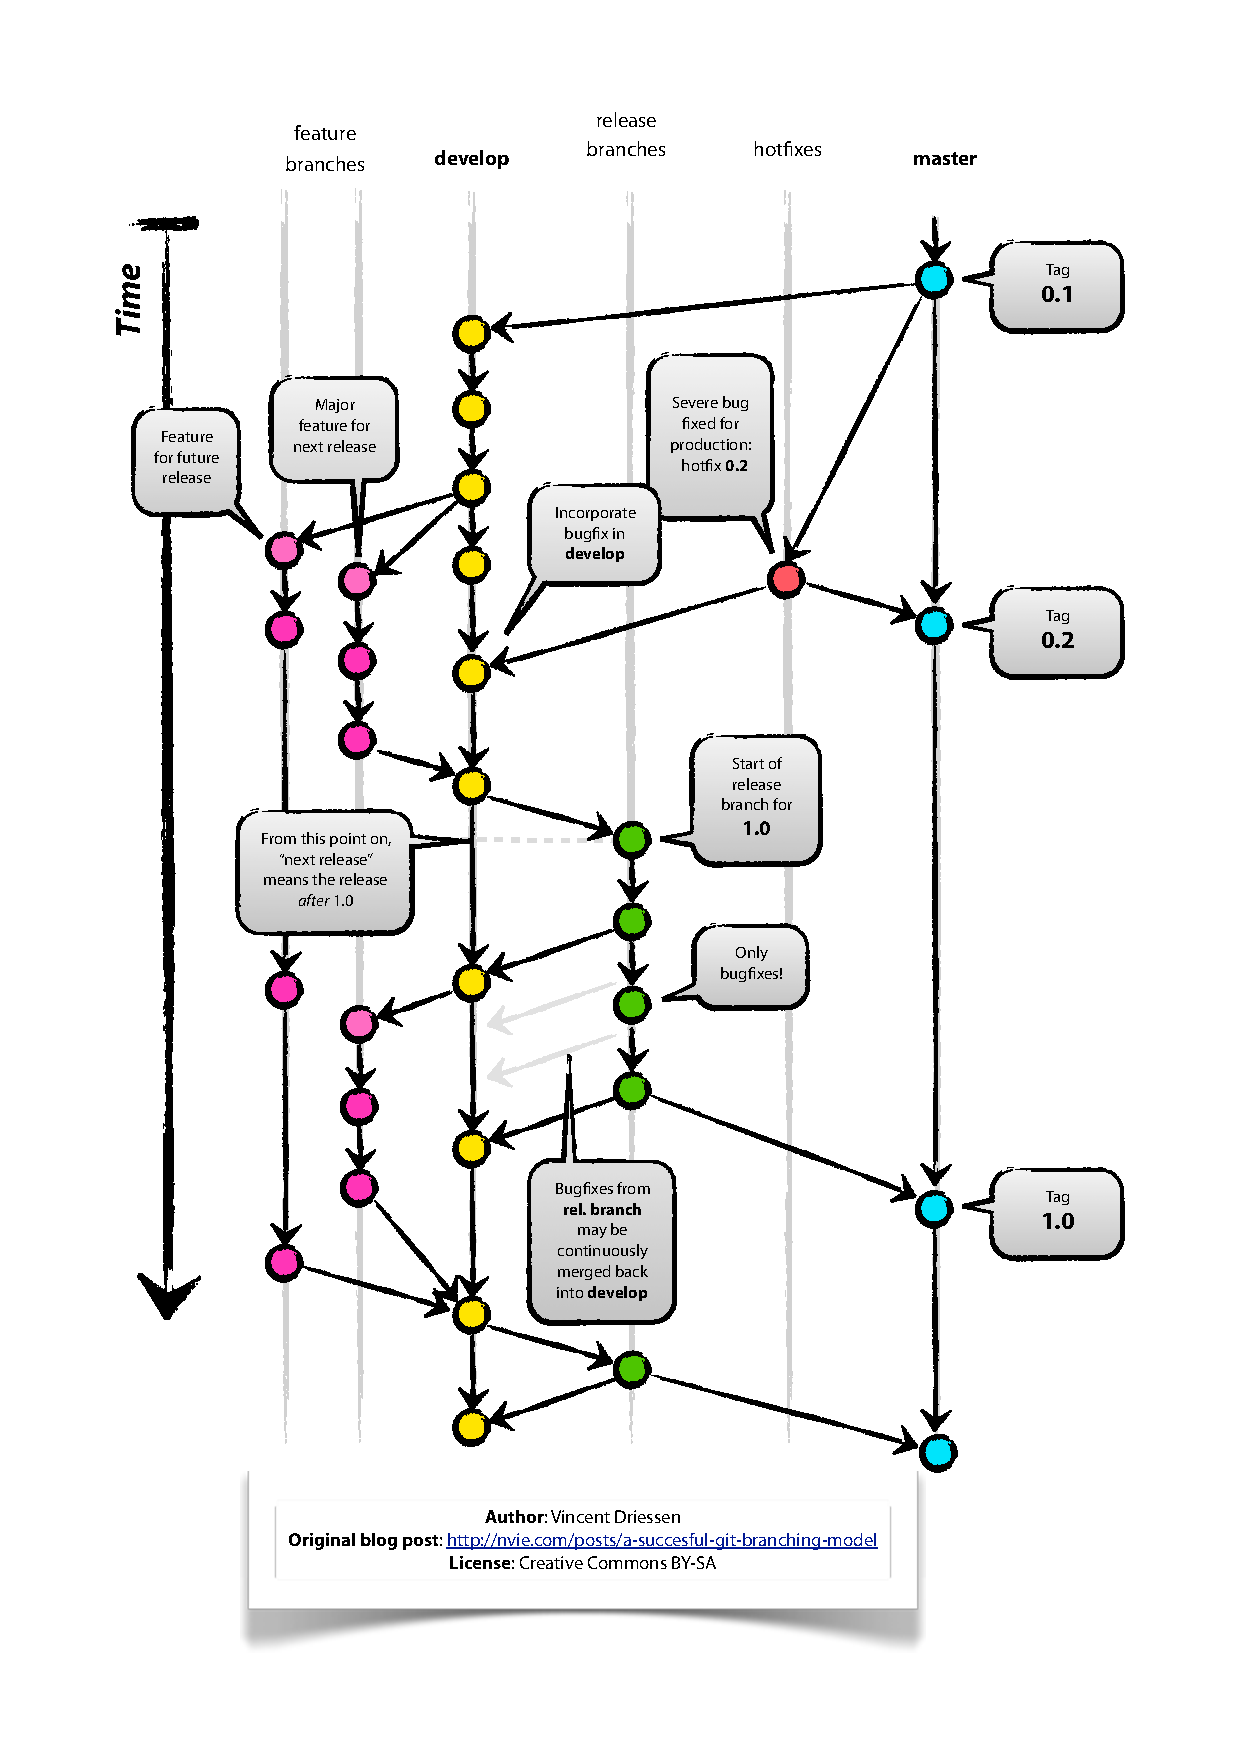
\includepdf[pages={1}]{Git-branching-model.pdf}

\end{document}
